The third question of the survey asks participants about their choice of presentational design patterns. In this question, MVVM, MVP, MVI, etc. design patterns were defined as presentational design patterns. When the results are  examined, a diverse set of answers is seen. Below, in Fig. \ref{fig:design_pattern} the participants' preferences for presentational design patterns are displayed.
\begin{figure}[ht!]
    \centering
    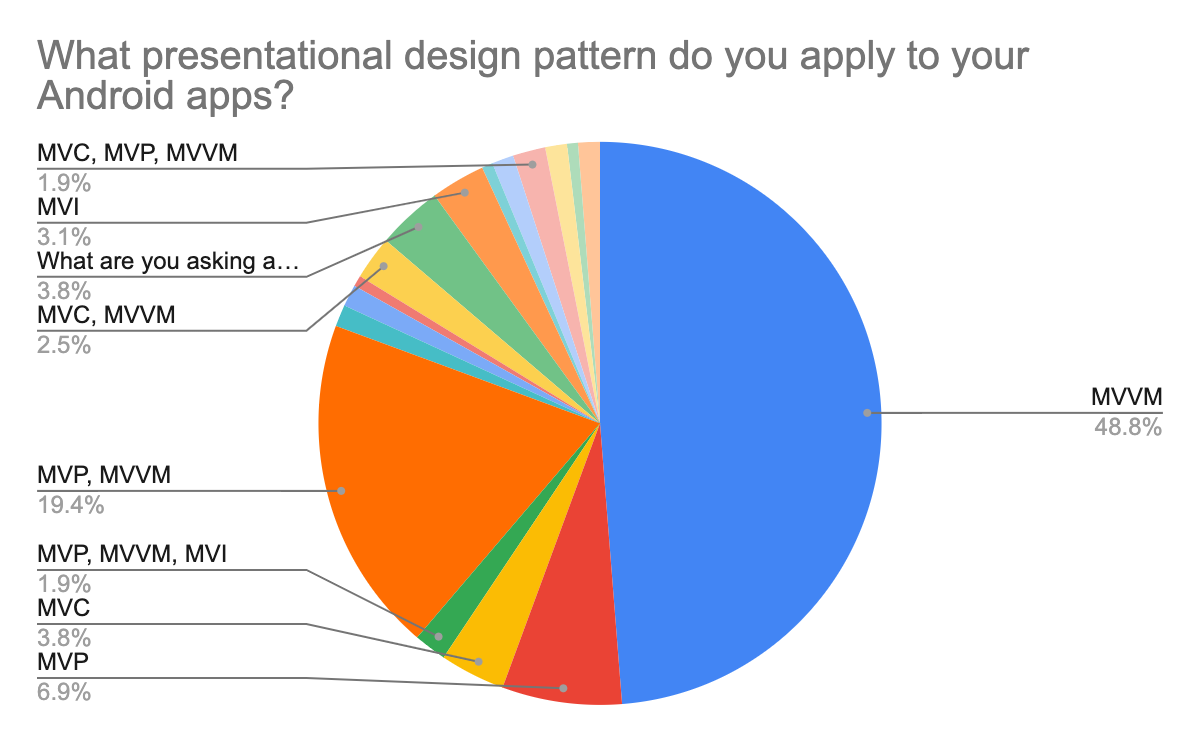
\includegraphics[scale=0.3]{figures/survey_q3_design_pattern.png}
    \caption{Presentational design patterns results}
    \label{fig:design_pattern}
\end{figure}
\FloatBarrier
The first notable conclusion is that almost half of the participants use the MVVM presentational design pattern. Besides, it is seen that another 25\% of the participants stated that they used this design pattern and different design patterns. In other words, a total of 3 quarters of the participants stated that they used the MVVM design pattern in some way or another. On the other hand, the chart presents us that design patterns such as MVP, MVC, MVI are also frequently used. When the participants' responses are sifted through, it is seen that design patterns such as MVP, MVC and MVI are generally preferred by some developers alongside the MVVM design pattern. These developers have more experience than those who have a single choice of design pattern. Also, it was seen that developers with 0-3 years of experience have answered this question by selecting the MVVM option. Another important detail is that 5 out of 6 participants that answered this question as "What are you asking about" had one year or less experience. Lastly, it was seen that the MVI design pattern was selected nine times in the last six months (out of 120 answers with a ratio of 0.075). However, it was selected only once (out of 40 answers with a ratio of 0.025) by the participants in the first six months in which the survey accepted answers.

In the following question, users were asked whether they use the "Clean Architecture". It is essential to mention why Clean Architecture was asked to the participants differently from the presentational design patterns. Clean Architecture allows the arrangement of an entire application in terms of architecture, unlike the presentational design patterns. The graphical breakdown of participant answers to this question is presented below in Fig \ref{fig:clean_arch}.
\begin{figure}[ht!]
    \centering
    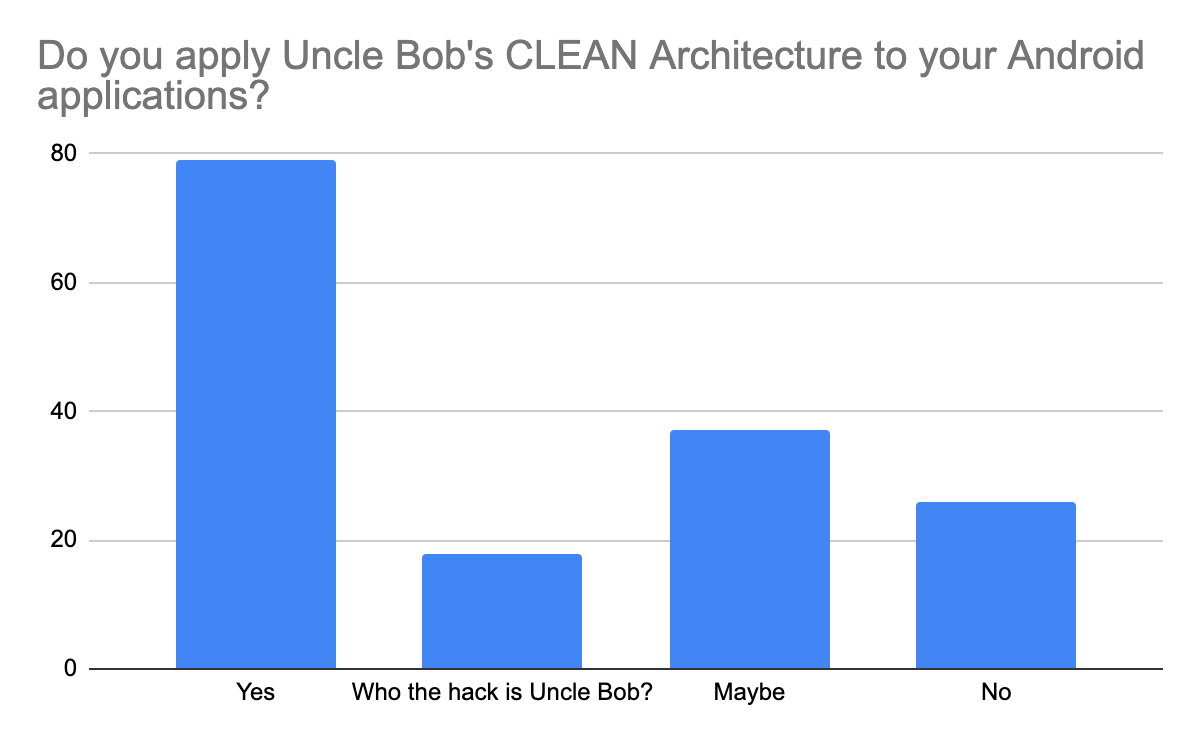
\includegraphics[scale=0.33]{figures/survey_q4_clean_arch.png}
    \caption{Clean Architecture usage results}
    \label{fig:clean_arch}
\end{figure}
\FloatBarrier

When examining the participatory tendencies to use Clean Architecture, it is seen that the majority of the participants adopt this architectural approach. The number of respondents who declared their use of this architectural pattern is almost more than the total of those who declared that they did not or could use it. Besides, 38 of 51 Android developers with five or more years of experience who participated in the survey declared that they use or can use this architectural pattern.